% !TEX encoding = UTF-8
% !TEX TS-program = pdflatex
% !TEX root = ../tesi.tex
\begin{usecase}{5}{Upload Dati}
  \usecaseactors{Utente autorizzato}
  \usecasepre{Lo sviluppatore è entrato nel plug-in di simulazione all'interno dell'IDE}
  \usecasedesc{La finestra di simulazione mette a disposizione i comandi per configurare, registrare o eseguire un test}
  \usecasepost{Il sistema è pronto per permettere una nuova interazione}
  \label{uc:upload-dati}
\end{usecase}

\subsection{UC5 - Upload procedimento}
\begin{itemize}
  \item \textbf{Identificativo}: UC5
  \item \textbf{Nome}: upload procedimento
  \item \textbf{Descrizione grafica}:
\end{itemize}

\begin{figure}[h]
  \centering
  %  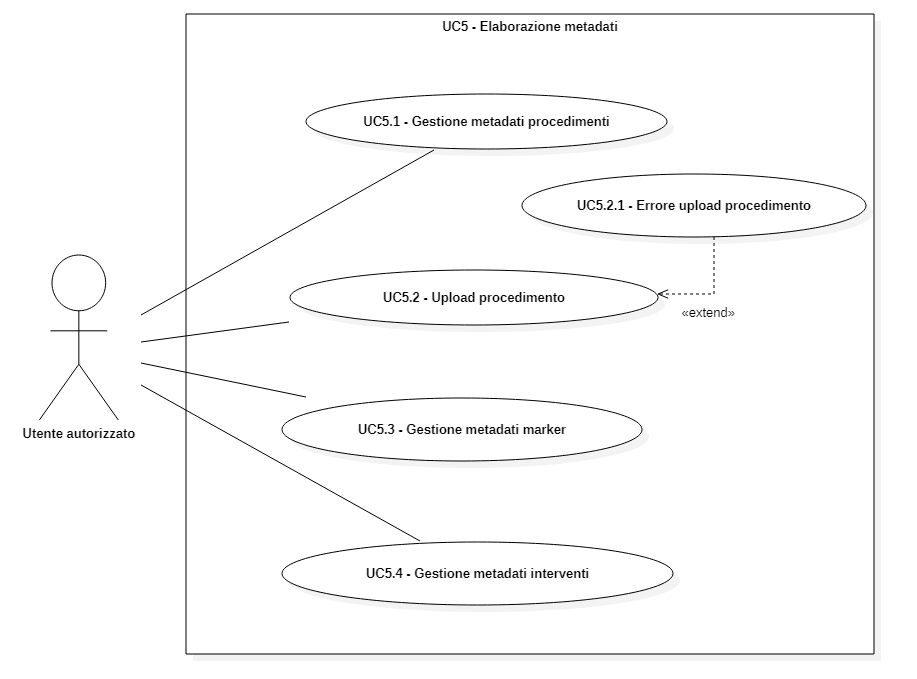
\includegraphics[scale=0.50]{images/UC5.png}
  \caption{Descrizione grafica caso d'uso UC5}
\end{figure}

\begin{itemize}
  \item \textbf{Attori}
        \begin{itemize}
          \item \textit{Primari}: utente autorizzato
        \end{itemize}
  \item \textbf{Precondizione}: l'utente si trova sulla pagina di visualizzazione dei dati.
  \item \textbf{Postcondizione}: l'utente ha caricato il procedimento desiderato e i relativi file.
  \item \textbf{Scenario principale}: l'utente tramite l'apposito bottone per l'upload, carica il procedimento desiderato.
  \item \textbf{Scenario secondario}: la procedura di upload procedimento non va a buon fine e restituisce un errore. (\textbf{UC5.1})
\end{itemize}

\subsubsection{UC5.1 - Errore upload procedimento}
\begin{itemize}
  \item \textbf{Identificativo}: UC5.1
  \item \textbf{Nome}: errore upload procedimento
  \item \textbf{Descrizione grafica}: (approfondita in UC5)
  \item \textbf{Attori}
        \begin{itemize}
          \item \textit{Primari}: utente autorizzato
        \end{itemize}
  \item \textbf{Precondizione}: il sistema non ha gestito correttamente la richiesta di upload procedimento.
  \item \textbf{Postcondizione}: l'errore viene visualizzato sull'applicazione.
  \item \textbf{Scenario principale}: la richiesta di upload procedimento non va a buon fine e l'errore viene mostrato all'utente.
\end{itemize}
